\begin{document}

\flushbottom % Makes all text pages the same height

\maketitle % Print the title and abstract box

\tableofcontents % Print the contents section

\thispagestyle{empty} % Removes page numbering from the first page

%-
%	ARTICLE CONTENTS
%-

\section{Overview} % The \section*{} command stops section numbering
\addcontentsline{toc}{section}{Introduction} % Adds this section to the table of contents
This document describes the basic client software required to transmit and receive CCN messages
via CCN Forwarders on a CCN Network. As shown in Figure 1, an application may use the Portal API to manipulate 
the Transport Stack to send and receive messages on a CCN network.

 \begin{figure}[ht]
\center{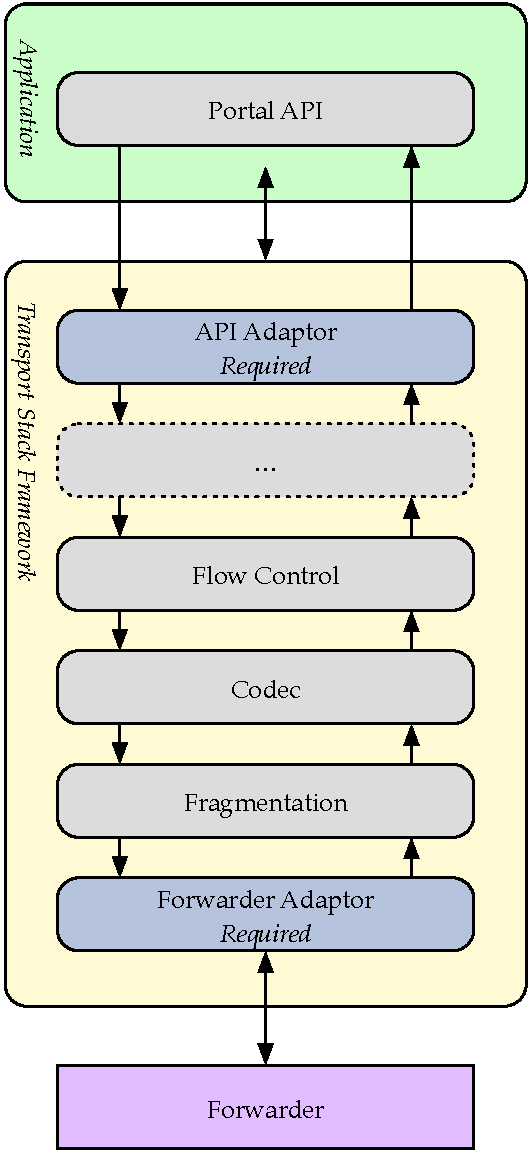
\includegraphics[width=205pt]{StackDiagram}}
\caption{Transport Stack ({\it typ.\/})}
\end{figure}


The Transport Stack is composed of a set of components, each focused on a specific task. Typical stacks include components
for CCN Flow Control, outbound message signing, inbound message signature verification,
packet format encoding and decoding, fragmentation and reassembly, and CCN Forwarder communication.
The extensible architecture supports stacks from the very primitive, providing only  mandatory features such as datagram-style message sending and receiving, to the highly sophisticated, providing optional features such as an in-order stream of Content Objects with arbitrary rewind and fast-forward within the stream.  Different Transport Stacks may include different features of different implementations of the same
features.

The Portal API provides a simple interface to the Transport Stack allowing the application to compose, use, and maintain Transport Stacks and to perform message operations through the stack. Each Portal API instance is associated with a specific CCN Transport Stack.
It is a low-level API providing a simple interface upon which applications and other interfaces are implemented. Examples of higher level services that could leverage the Portal API include the CCN Assembly Framework, the CCN Key-Value Store API, and the CCN Message Queue API.

Together, the Portal API and its associated Transport Stack provide the basic mechanism for sending and receiving CCN messages. These Messages contain Interests, Content Objects, and Control messages.
Interests and Content Objects are the primary elements of discourse in CCN,
while Control messages govern the operation of various network elements. 
Taken together, the combination of Portal API associated with a Stack is called a Portal instance. 
The Portal instance is a library of functions that perform operations between the API and the Stack.
The CCN Portal library creates, maintains, and uses CCN Portal API instances.

\section{Requirements}

\subsection {The Transport Stack}
The Transport Stack must:
\begin{itemize}
\item provide a full interface for the CCN Portal API to access.

\item isolate specific technical concerns into distinct functional components with different experimental and non-experimental implementations.

\item isolate implementation details for encoding and decoding of network packets,
signing and verification,fragmentation and reassembly, flow and rate control from the application's concern.

\item be able to easily interface with multiple kinds of CCN Forwarder implementations.

\item be easily extensible and a good platform for experimentation.
\end{itemize}

\subsection {Portal API}
Each Portal API must:

\begin{itemize}
\item be able to compose,
instantiate, associate with, and ultimately use a single
Transport Stack instantiation using the Transport Framework API.

\item be bound to an identity representing the Portal API instance and its Transport Stack.

\item provide transmission and reception of individual CCN Messages (e.g. Interest, Content Object, and Control messages).

\item provide support for the establishing and abolishing in-bound reception of CCN Messages based upon a CCN Name.

\item provide a facility to set and get attributes related to the state and operation of the Portal instance and its associated Stack. Attributes include:
\begin{itemize}
\item an indication of whether dynamically modifiable blocking or non-blocking modes of reception and transmission are used.

\item an indication that a stack will no longer provide or accept inbound or outbound CCN Messages.
\end{itemize}

\end{itemize}
\section{Transport Stack}
The Transport Stack is a component based piece of software following the chain-of-command pattern. It manages two message queues: 
\begin{itemize}
\item An outbound queue moving messages from the application toward the network.
\item An inbound queue moving messages from the network toward the application.
\end{itemize}

As shown in figure 1, The Transport Stack is composed of a set of optional components and two required components: the API Adaptor and the Forwarder Adaptor.  Messages are pipelined through the Transport Stack components on their way between the Portal API and the Forwarder.  Possible stack components might include elements to handle fragmentation, codecs to translate a programmatic representation of a message into a properly encoded packet, flow control components to manage prefetching, or any other component implemented by a third party.  The Transport Stack is designed to be extensible such that an application can utilize as simple or as a sophisticated set of components as it needs.

An application uses the Portal API instance to create, manipulate, and use a Transport Stack.
The Portal API sends and receives messages through the Transport Stack's API Adaptor.

\subsection{Transport Stack Names}
The Portal API can reference its own Transport Stack by the name "localstack" in order to set or get properties in the Transport Stack's management information database. This name is valid only within the scope of a single Transport Stack.

A Transport Stack may also have a name assigned to it by its Forwarder Adaptor.
This name distinguishes one Transport Stack from another within the scope of a single Forwarder.

\subsection{Transport Stack Components}
A Transport Stack is composed of a set of components through which messages flow in both inbound and outbound directions.
Each component focuses on a single purpose, thus maintaining a separation of concerns between elements in the stack, and enabling a 
plug-and-play approach to stack composition for different needs.

The following descriptions illustrate typical components in the Transport Stack. 
It is not an exhaustive list, and only the API adaptor and Forwarder Adaptor are required. 

\subsubsection{API Adaptor}
The API adaptor is a required component providing the interface
between the stack and the application's Portal instance.
At a minimum, it translates messages between the execution environments of the application and the stack.

\subsubsection{Flow Control}
The Flow Control component is an optional component
responsible for managing the flow of outbound and inbound messages to
ensure in-order delivery, retransmission, sequential fetching and prefetching of messages.

\subsubsection{Codec}
The Codec component translates a programmatic form of a message into a properly formatted packet suitable for transmission and vice-versa.

The message signature computed over the formatted byte array requires the Codec component to have access to encryption keys for signing and verification.
This access is provided to the Codec component in any way suitable for the implementation.
For example, a Codec component implementation might use an identity framework external to the Stack,
it might participate in a protocol to fetch identity information from the network,
or it might simply be provided with the identity information from the Portal API via a Control message.

\subsubsection{Fragmentation}
Fully formatted packets may exceed the size of a maximum transfer unit and as a consequence
must be fragmented for transmission.
Similarly, when fragments are received, they must be reassembled into fully formed packets.

\subsubsection{Forwarder Adaptor}
The Forwarder Adaptor is a required component providing the interface between the Stack and the CCN Forwarder.
The Forwarder Adaptor is responsible for establishing an association with a CCN Forwarder
and interacting with the Forwarder to transmit and receive network packets.

For example, a Forwarder implementation may execute on a computer and communicate with all of the Forwarder Adaptors via an IPC mechanism.
In this case, the Forwarder Adaptor establishes the IPC channel with the Forwarder.
Similarly, the Forwarder may provide administrative controls out-of-band from the packets it receives. In this case the Forwarder Adaptor is responsible for using those out-of-band controls as necessary.

\subsection{Future}
The Transport Stack architecture is illustrative but not entirely prescriptive.
Over time, we expect that well-known, canonical, stack ensembles will emerge
that are no longer concerned with extensibility or experimentation.
It would be reasonable to implement such ensembles in as few components as necessary, to promote consistency and ease-of-use.
Nevertheless, even those omnibus components should be designed with the same requirements for separation of concerns and ease of extensibility or maintenance in mind.

\section{Transport Framework}
The Transport Framework is responsible for supplying the runtime environment for a Transport Stack.
It provides an interface for composing and decomposing Transport Stacks and interfaces with the 
necessary system resources (e.g. the operating system, communication interfaces, etc.). While an application
may start multiple Portal instances with associated Transport Stacks, it will only have one Transport Framework
to manage all stacks.

\begin{figure}[ht]
\center{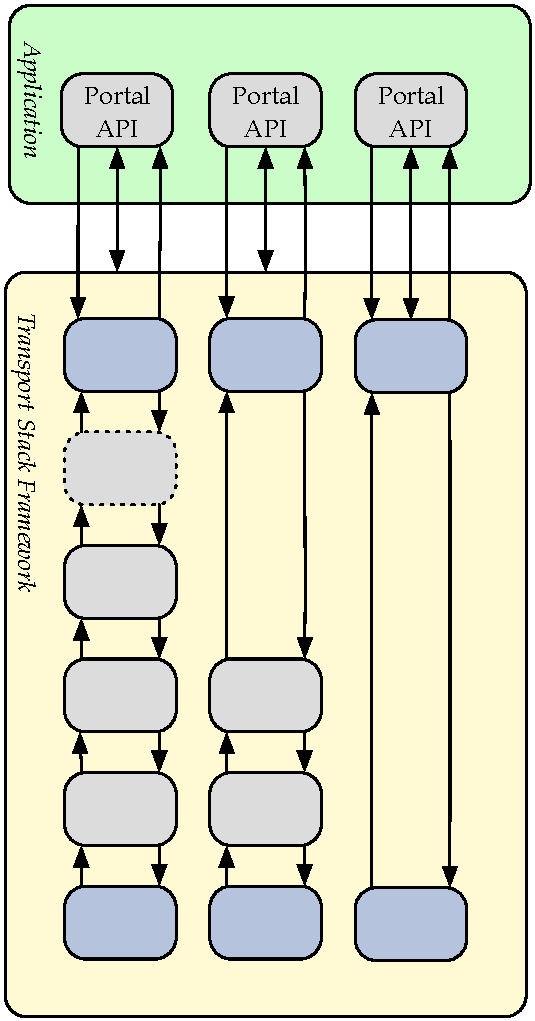
\includegraphics[width=205pt]{TransportStackFramework}}
\caption{A Transport Framework with multiple, different Transport Stacks.}
\end{figure}

\section{Portal Instances}
When a Portal instance is created, it is immediately associated with a Transport Stack
*{\it under the auspices of a specific identity}.

In this case, the identity is a digital representation of an entity such as an individual, an organization,
an administrative function, etc.
The identity should not be confused with a CCN {\it Name} which is a label for something to which messages can be sent, although in some cases
CCN Named entities may also serve as the identity context of a Portal instance. 

\noindent\fbox{\parbox{\textwidth/2 -5\fboxsep-2\fboxrule}{
{\it *This identity represents the creator of the Stack, which may not necessarily represent the user of the stack.
For example, an administrative function may create a specific Stack using an administrative identity,
providing necessary authentication to other services that assist in the creation of the Stack
then delegate the use of the Stack to an application that does not possess those administrative credentials.}}}

During the course of the Stack's creation and its binding with the Portal instance,
the Stack acquires a unique CCN LCI name colloquially called "{\tt localstack}". This uniquely identifies the Portal-Stack assembly.
As a matter of convenience, a specific label from the Labeled Content Information schema is used as shorthand for {\tt localstack}.

A CCN Transport Stack is comprised of multiple components forming a chain-of-command pattern to send and receive CCN messages.
The formulation of a Stack is prescribed by the Portal instance itself when it is created. For example, Portal instances providing message-by-message-like behavior will create and associate with a Transport Stack providing such behavior; 
Portal instances providing in-order delivery of Content Object messages, being triggered by an initial Interest message,
will create and associate with a Transport Stack containing components to implement that behavior.

When the life of a CCN Portal instance has ended,
it is released by its application and resources are deallocated by the operating environment's runtime normally.

Application interactions with the Portal instance consist of invoking methods to send or receive CCN Messages, get or set meta-data regarding the state of the Portal instance.

\subsection{Portal Attributes}
Transport Stacks are composed of multiple components,
 each with potentially different attributes that together
indicate the current state of the stack. 
Each Portal instance maintains a common interface to these attributes.
 
Some attributes are read-only (for example, a flow control component will signal the state of the flow in a read only attribute),
while others may be modified only by their specific component (for example, the application specifies blocking or non-blocking modes
through a read-write attribute).


\subsubsection{Queueing Modes}

\begin{enumerate}
\item {\bf Blocking}
The client of the Portal instance will block on operations that require a Message to be sent or received if sufficient resources are unavailable.
\item {\bf Non-blocking}
The client of the Portal instance will not block on operations that require a Message to be sent or received earn sufficient resources are unavailable.
\end{enumerate}


\subsection{Methods}
Once a Portal instance is created,
CCN Messages are sent and received via the appropriate API methods as listed below.

\subsubsection{Send}

The {\tt Send} method enqueues a CCN Message on the outbound queue.

If the queuing mode of the Portal instance is non-blocking and the outbound queue is full,
this method will fail and signal failure without changing the state of the Portal instance.

If the queuing mode of the Portal instance is blocking and the outbound queue is full,
this function will block until it is able to successfully enqueue the Message to send.

\subsubsection{Receive}

The {\tt Receive} method dequeues a CCN Message from the inbound queue in the Transport Stack.

If the queuing mode of the Portal instance is non-blocking and the inbound queue is empty,
this method will fail and signal a temporary failure.

If the queuing mode of the Portal instance is blocking and the inbound queue is empty,
this function will block until it is able to successfully dequeue a Message to send. {\bf should this be receive?}

\subsubsection{Get Identity}
Return the Identity associated with the Portal instance.

\subsubsection{Set Identity}
Set the Identity associated with the Portal instance.
Setting the Identity does not change the name of the Portal instance. {\bf what is the name?}

\subsubsection{Get Attribute}
Fetch the value of a named attribute maintained by the Portal instance and its associated Transport Stack.

\subsubsection{Set Attribute}
Set the value of a named attribute maintained by the Portal instance and its associated Transport Stack.
The Set is a compare-and-swap wherein a predicate value for the attribute is supplied and if the predicate value 
is equal to the current value of the attribute,
the attribute value is set to the new value.  

\subsubsection{Listen}
A convenience method that sends the correct Control message to cause CCN Interests with Names starting with a specific prefix to be enqueued in the Transport Stack input queue.
This operation may require authorization. {\bf why is this a convenience method?  Isn't listening and ignoring the main thing to do? who provides authorization}

\subsubsection{Ignore}
A convenience method that send the correct Control message to cause CCN Interests for Names starting with a specific prefix to not be enqueued in the Transport Stack input queue.

\section{CCN Messages}
CCN Messages are Interests, Content Objects, and Control messages.
Each messages contains a CCN Name that directs where the message is sent.
For example, a CCN Interest message follows the path defined in the Forwarding Information Base (FIB) and deposits an entry in the Pending Interest Table (PIT) of the Forwarder.
A CCN Content Object messages follows the reverse path specified in the PIT entry and consumes the entry.

\subsection{Interest}
An Interest is a CCN Message requesting the CCN Content Object message (matching the Name specified in the Interest message) as a response.

\subsection{Content Object}

A Content Object is a CCN Message response to a received CCN Message request.

\subsection{Control}
Control messages direct the operation of the Portal instance,
the Transport Stack, and the local Forwarder. They are delivered in the order received by the API or Forwarder Adaptors.

Control Messages are directed to a specific component in a stack by including the LCI name of the component in the message.  The Name is a composite of the stack name and the name of a component. For example, a message addressed to the Name {\tt lci:/localstack/codec} would be directed to the {\tt codec} component in the Transport Stack.  Every Control message request results in a Control message response. The following section outline a typical set of messages for various Transport Stack components.

{\it 
Notifications as we have them now are just Control messages "up-side-down,"
or "inbound" rather than outbound.
A notification is just an unexpected inbound message signalling some state change or information
(usually after the fact).
Similarly the control messages are outbound,
just as unexpected and signal some state change or information
(usually before the fact).
So a notification can just be a Control message going the other way.

If we do away with special messages for notifications and special cases for their behavior,
and reuse the Control Message as both an outbound and inbound message, then the inbound (notification) would require a response.
But that could be a function of the Portal API library which,
when it receives an inbound control message always responds with an ACK,
plus it maintains a representation of the state of the Stack anyway so this is good.

That would have interesting effects:
I could formulate a control message in my application.
Send it via Portal down my Transport Stack, through the forwarder to another stack.
That stack would then receive my control message, possibly act upon it and send a reply.
Yes I'm skipping over the authorization and authentication part,
I expect them to be there but I don't expect to always have to describe them.

But at this point, it looks like a CCN Interest again.
So control messages and notifications just more Interests and Content Objects?
Or they are Interests and Content Objects with special cased behavior?
}


{\it I make a distinction between Control Messages that affect the stack those that may be transmitted on the network.  This is only for clarity at the moment, it may be that they are the same thing, just distinguished by "scope."}

\section{Control Messages for Stack Components}
\subsection{API Adaptor Control Messages}
{\tt lci:/localstack/api}

\subsubsection{Pause}
Cause the API Adaptor and each component subsequently receiving this message
on the outbound-side of the Stack to not accept any new outbound messages.
The Forwarder Adaptor must reply to this message and prohibit the enqueing
of any new inbound message.
The Forwarder Adaptor's reply indicates to each inbound component
to not accept any new inbound messages that are not reply messages.

\subsubsection{Resume}
Cause the API adaptor and each subsequent component to accept new outbound messages,
The Forwarder Adaptor must reply to this message and enable the enqueing of new inbound messages.
The Forwarder Adaptor's reply indicates to each inbound component to accept new inbound messages.

\subsubsection{GetAttributes}
Get the attributes of the API Adaptor Component.

\subsection{Flow Control Control Messages}
{\tt lci:/localstack/flowcontrol}

The Flow Control component manages the transmission and reception of data comprised of many,
in-order messages.

A flow is started as the result of the Flow Control component
receiving an Interest message with the Name containing a valid chunked specification.
The current position of the flow is set to the value of the chunk
specified and the limit is set to infinity.

{\it Need a way to name a flow.}

\subsubsection{StartFlow}
Signal the Flow Control component to start a flow from a specific position to a limit.
When the flow reaches the limit,
an inbound message is enqueued signaling that the flow terminated because it reached the limit.
If the flow terminates before reaching the limit,
an inbound notification message is enqueued signaling that the flow terminated normally.

\subsubsection{GetPosition}
Get the current position of the specified flow.

\subsubsection{SetLimit}
Signal the Flow Control component to immediately set the current limit to the given value.
The limit can never be set less than the current position.

\subsubsection{GetLimit}
Get the current limit of the flow.

\paragraph{StopFlow}
Signal the Flow Control component to immediately stop a flow.

\subsubsection{GetAttributes}
Get the attributes of the Flow Control Component.

\subsection{Signing Component Control Messages}
{\tt lci:/localstack/signing}

\subsubsection{SetKey}
Set the signing key for all subsequent messages.

\subsubsection{UnsetKey}
Remove the signing key for all subsequent messages.
Depending upon the implementation behavior of the Signing Component,
this may cause unsigned messages to be transmitted,
or the Signing Component may block and signal errors until a new key has been set.

\subsubsection{GetAttributes}
Get the attributes of the Signing Component.

\subsection{Verification Component Control Messages}
{\tt lci:/localstack/verification}

\subsubsection{AddKey}
Add a verification key to the set of keys for valid inbound messages.

\subsubsection{DeleteKey}
Delete a verification key from the set of keys for valid inbound messages.

\subsubsection{GetAttributes}
Get the attributes of the Verification Component.

\subsection{Fragmentation Component Control Messages}
{\tt lci:/localstack/fragmentation}

\subsubsection{GetFragmentSize}
Get the current Fragment Size used by the Fragmentation Component.

\subsubsection{SetFragmentSize}
Set the current Fragment Size used by the Fragmentation Component.

\subsubsection{GetAttributes}
Get the attributes of the Fragmentation Component.

\subsection{Forwarder Adapter Control Messages}
{\tt lci:/localstack/forwarder}

\subsubsection{CreateRoute}
Create a FIB entry for the given name to a specified interface.
The entry must not already exist.
This operation may require authorization.

\subsubsection{ReadRoute}
Fetch the FIB entry for the given name.
If the name does not exist, the reply indicates failure.
This operation may require authorization.

\subsubsection{UpdateRoute}
Modify an existing FIB entry for a given name.
An existing FIB entry must already exist.
This operation may require authorization.

\subsubsection{DeleteRoute}
Delete an existing FIB entry for a given name.
If the name does not exist, the reply indicates failure.
This operation may require authorization.

\subsubsection{GetRoutes}
Fetch information about all of the FIB entries in the Forwarder visible by this Portal Stack.
This operation may require authorization.

\subsubsection{GetInterfaces}
Fetch information about all interfaces visible by this Portal Stack.
This operation may require authorization.

\subsubsection{Listen}
Direct the Forwarder to forward CCN Interests with names starting with a specific prefix to this Portal Stack.
The Forwarder adaptor enqueues these messages in the Transport Stack input queue.
This operation may require authorization.

\subsubsection{GetAttributes}
Get the attributes of the Forwarder Adaptor.

\subsubsection{Ignore}
Direct the Forwarder to not forward CCN Interests with names starting with a specific prefix to this Portal Stack.


%
%\subsubsection{Request}
%Request Control messages are either a query or a query/update for state and configuration information for the one or more network elements.
%
%For example, a Control message could request the KeyId used by Portal and its associated stack for signing outbound Content Objects.
%Similarly, a Control message can request the KeyId used by Portal and its associated stack to be changed.
%
%\subsubsection{Response}
%Every Request Control Message produces a Response Control Message which is sent upwards to the Portal to be either read and interpreted by the Portal API implementation, or passed to the client of the Portal API for processing.
%A Response Control Message indicates either success or failure of the original Request Control Message.
%
%\subsubsection{Close}
%
%\subsubsection{Add Route}
%
%\subsubsection{Add Route To This Stack}
%
%%------------------------------------------------
%
%\section{Implementation}
%
%A CCN Portal instance is created either by the CCN Portal Factory,
%which is a generator of CCN Portal API instances sharing a common set of attributes held by the factory,
%or by creating the CCN Portal API instance directly by calling its creation method.
%
%\section{Discussion}
%
%\subsubsection{Multiple Identities}
%An example use has been noted where there is a single Portal on which
%Content Objects to send are to be signed by different keys.
%A prerequisite for this is for the signing component in the Transport Stack to change the key used to sign Content Objects as they are encoded.
%
%Thus, the Portal use would consist of sending a Control Message setting the signing key and sending Content Objects.
%When a Content Object must be sent signed by a different key, the application uses Portal to send a Control Message setting the new signing key and sending the Content Objects.
%
%This has an impact on the semantics and implementation of {\tt GetKeyId} for the Portal instance.
%For example, does GetKeyId return the KeyId of the current KeyId being used by the Transport Stack's signing component, or does it return the in the most recent Change Key Control message?
%

%------------------------------------------------
%\phantomsection
%\section*{Acknowledgments} % The \section*{} command stops section numbering%
%
%\addcontentsline{toc}{section}{Acknowledgments} % Adds this section to the table of contents



%----------------------------------------------------------------------------------------
%	REFERENCE LIST
%----------------------------------------------------------------------------------------
\phantomsection
%\bibliographystyle{unsrt}
%\bibliography{sample}

%----------------------------------------------------------------------------------------

\end{document}
